\documentclass[a4paper, oneside]{book}
\usepackage{CJKutf8}
\usepackage{indentfirst}
\usepackage{graphicx}
\usepackage{multirow}
\usepackage{verbatim}
\usepackage[unicode=true]{hyperref}


\renewcommand{\tablename}{表}
\renewcommand{\figurename}{图}

\author{The Cytoscape Collaboration \\ Translated by Gang Chen}
\title{Cytoscape用户手册}
\date{\today}

\begin{document}
\begin{CJK}{UTF8}{msyh}
\maketitle
\tableofcontents

\chapter*{Cytoscape 2.6用户手册}
本文档遵守Creative Commons License,2006

作者:The Cytoscape Collaboration

中文翻译:Gang Chen <chengang@gossipcoder.com>

Cytoscape项目由以下单位合作:
\begin{itemize}
\item 加州大学圣地亚哥分校
\item 系统生物学研究中心
\item Memorial Sloan-Kettering癌症研究中心
\item Pasteur研究中心
\item 安捷伦科技公司
\item 加州大学旧金山分校
\end{itemize}

Cytoscape的资金来自NIH的美国国家通用医学研究中心(NIGMS),资金编号为:GM070743-01。整体资金通过来自Unilever PLC的合同提供。

\chapter*{引言}
Cytoscape~项目致力于为用户提供一个开源的网络显示和分析软件。软件的核心部分提供了网络显示、布局、查询等方面的基本功能。软件的核心可以通过插件架构进行扩展,这样就能快速地开发出新的功能。

Cytoscape源自系统生物学,用于将生物分子交互网络与高通量基因表
达数据和其他的分子状态信息整合在一起。虽然Cytoscape也能适用于
其他分子构件和相互作用,但其最强大的功能还是用于大规模蛋白质-
蛋白质相互作用、蛋白质-DNA和遗传交互作用的分析。各种物种,包括
人类,的这方面的实验数据都在迅速增加。通过Cytoscape,用户可以在可视化
的环境下将这些生物网络跟基因表达、基因型等各种分子状态信息整合
在一起,还能将这些网络跟功能注释数据库链接在一起。

Cytoscape~的核心是网络(图),其中的节点(~node~)是基因、蛋白质或分子,其中的连接则是这些生物结构之间的相互作用。

\section{开发}

Cytoscape~是~Institute for Systems Biology~(~Leroy Hood~实验室)、加州大学圣地亚哥分校(~Trey Ideker~实验室)、~Memorial Sloan-Kettering~癌症研究中心(~Chris Sander~实验室)、Pasteur研究院(Benno Schwikowski实验室)、安捷伦科技(Annette Adler实验室)和加州大学旧金山分校(Bruce Conklin实验室)的合作项目。

详情请访问http://www.cytoscape.org。

\section{授权}
Cytoscape~受~GNU LGPL~(~Lesser General Public License~)~的保护。在本手册的附录中能找到该授权,同时可以访问~http://www.gnu.org/copyleft/lesser.txt~。~Cytoscape~还是用了其他的一些开源程序库,详情见本手册的致谢。

\section{2.6版本的更新}
Cytoscape 2.6~中增加了很多新功能,在性能和软件的易用性上也有提升。包括:
\begin{itemize}
\item Web Service Client Manager框架能将Web服务客户端集成到Cytoscape中。
\item 通过Web服务客户端插件,可以从PathwayCommons、IntAct和NCBI Entrez Gene下载网络数据。
\item 通过Web服务插件,可以从BioMart导入注释信息。这主要是用于ID的翻译和名称映射。
\item Cytoscape主题。
Dynamic filters.
\item 动态过滤器。
Network Manager supports multiple network selection.
\item 网络管理器支持多网络选取。
Label Positioning has been improved.
\item 改进了标签的位置。
Session saving occurs in memory.
\item 将会话保存在内存中。
XGMML Improvements.
\item 改进了XGMML。
Network loading improvements.
\item 网络加载得到了改进。
\item Linkout integrated with attribute browser.
\item 通过可视化属性,引入了更多的Visual Style。
\item 修复了不计其数的bug。
\end{itemize}


\chapter{启动~Cytoscape}
Cytoscape~是一个Java程序,能在~Linux~、~Windows~和~Mac OS X~上运行。对于其他能安装Java 5的操作系统平台,比如以Solaris和FreeBSD为代表的UNIX,Cytoscape也能运行,但官方并对此提供支持。

\section{系统要求}
	Cytoscape~对系统的具体要求取决于所加载、查看和操作的网络的大小。

	\begin{table}[htbp]
	\label{tabel:2}
	\centering
	\begin{tabular}{|l|l|l|}
	\hline
	 & 小型网络查看 & 大型网络分析和查看 \\
	\hline
	处理器 & 1GHz & 尽可能的快\\
	\hline
	内存   & 512MB & 2GB以上 \\
	\hline
	显卡   & 板载集成显卡 & 高端独立显卡 \\
	\hline
	显示器 & XGA($1024 \times 768$) & 高分辨率或双显示器 \\
	\hline
	\end{tabular}
	\caption{}
	\end{table}

\section{入门}
	\subsection{安装~Java}
		如果计算机上还没有安装~Java,那么首先要下载并安装~Java SE 5~或~6~。\textbf{Cytoscape~从2.5版开始就不能在~Java 1.4~上运行。必须安装~Java SE 5~或~6~!!!}
		Java SE 5~和~Java SE 6可以从这里下载:
		\begin{itemize}
		\item \href{http://java.sun.com/javase/downloads/index_jdk5.jsp}{Java SE 5}
		\item \href{http://java.sun.com/javase/downloads/index.jsp}{Java SE 6}
		\end{itemize}
	
		一般情况下,Java SE 6~的运行速度要快一些。所以,如果您的计算机兼容~Java SE 6~的话,请尽量使用~Java SE 6。

	\subsection{安装~Cytoscape}
		Cytoscape~供下载的版本很多,安装方法也不尽相同。所有的版本都可以从~http://cytoscape.org~网站下载。
		
		\begin{itemize}
		\item Windows、Mac OS以及Linux平台上的自动安装包
		\item 压缩发行版
		\item 从源代码编译
		\item 从Subversion源中提取最新版的软件
		\end{itemize}

		Cytoscape的安装目录(无论是什么平台)中包含表~\ref{table:3}~中的文件。

		\begin{table}[!h]
		\begin{tabular}{|l|l|}
			\hline
			文件 & 描述 \\
			\hline
			cytoscape.jar & Cytoscape~的主程序(~Java~压缩包)。\\
			\hline
			\multirow{2}{*}{cytoscape.sh} & 从命令行运行~Cytoscape~的脚本(用于~Linux~和~\\&Mac OS X~)。\\
			\hline
			cytoscape.bat & 运行Cytoscape的脚本(用于~Windows~)。\\
			\hline
			LICENSE.txt/html & Cytoscape GNU LGPL~授权。\\
			\hline
			lib/ & Cytoscape运行所需的jar库。\\
			\hline
			docs/ & 各种格式的用户手册。也就是你正在阅读的东西。\\
			\hline
			plugins/ & jar格式的Cytoscape插件。\\
			\hline
			sampleData/ & \\
			\hline
				& galFiltered.gml -- 分子相互作用网络数据示例$^*$。\\
			\hline
				& galFiltered.sif -- Simple Interaction~格式的同一个网络$^*$\\
			\hline
				& galExpData.pvals -- 基因表达矩阵文件示例$^*$。\\
			\hline
				\multirow{2}{*}{} & galFilteredAttrTable.xls -- 微软~Excel~格式的节点属性\\ & 文件示例。\\
			\hline
				\multirow{2}{*}{} & galFiltered.sif -- 用上面的数据库和多个注释数据库创建\\ & 的会话示例$^*$。\\
			\hline
				\multirow{2}{*}{} & BINDyeast.sif -- BIND数据库中酵母的蛋白质相互作用\\ & 网络,2006年12月$^{**}$。\\
			\hline
				\multirow{2}{*}{} & BINDhuman.sif -- BIND数据库中人类的蛋白质相互作\\ & 用网络,2006年12月$^{**}$。\\
			\hline
				& yeastHighQuality -- 分子生物相互作用的示例文件$^{***}$。\\
			\hline
				\multirow{2}{*}{} & interactome\_{}merged\_{}networkTable.gz -- 制表符分割格\\ & 式的人类相互作用网络$^{****}$。\\
			\hline
				& sampleStyle.props -- 附加的~Visual Sytle~示例。\\
			\hline
		\end{tabular}
		\caption{$^*$ 来自~Ideker er al, Science 292:929 (2001); $^{**}$ 来自~http://www.blueprint.org/bind/bind\_{}downloads.html; $^{***}$ 来自~Mering et al, Nature, 417:399 (2002) Lee et al, Science 298:799 (2002);$^{****}$来自~Cytoscape~教程网页。原始数据可以从~http://cytoscape.org/cgi-bin/moin.cgi/Data\_{}Sets/上由Andrew Garrow、Yeyejide Adeleye和Guy Warner(Unilever, Safety and Enviromental Assurance Center)创建的“A merged human interactome”中下载。 }
		\label{table:3}
		\end{table}

	\subsection{启动程序}
		双击安装程序创建的图标,或是在命令行中运行~cytoscape.sh(Linux或Mac OS X),也可以双击~cytoscape.bat(Windows)~就能启动~Cytoscape。还可以在命令行中将这个jar文件以命令行参数的形式传递给命令~java -Xmx512M -jar cytoscape.jar -p plugins~。~-Xmx512M~标志是告诉~java~给~Cytoscape~分配较多的内存,~-p plugins~则是告诉~Cytoscape~加载~plugins~目录中所有的插件。插件对于~Cytoscape~是非常重要的,诸如布局(layout)、过滤器(filter)和属性浏览器之类的功能都是由插件提供的。关于命令行参数的详细信息请阅读\textit{命令行参数}一章。在~Windows~中,只需要双击~jar~文件就能启动~Cytoscape。不过,这样就不能使用命令行参数了(比如制定插件目录的位置)。

		成功地启动~Cytoscape后,就会看到如图~\ref{fig:1.1}~所示的窗口(图~\ref{fig:1.1}~来自Mac OS 10.4)。

		\begin{figure}[h]
			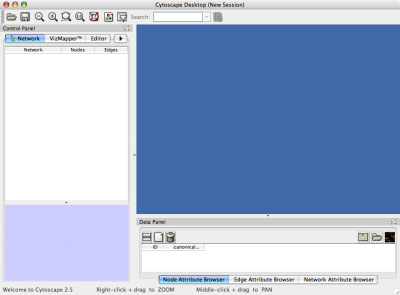
\includegraphics[width=\textwidth]{images/cytoscape_startup_mac.png}
			\caption{Cytoscape启动界面}
			\label{fig:1.1}
		\end{figure}

		\subsubsection{注意内存使用量}

		随着用用户所加载的网络的规模的增加,Cytoscape所需的内存也会增加。内存的使用量取决于网络对象(节点和边)的数量以及属性的数量。表~\ref{table:4}~和~\ref{table:5}是对内存需求量的粗略估计。

		\begin{table}[htbp]
		\centering
		\begin{tabular}{|l|l|}
			\hline
			对象的数量(节点和边) & 建议内存\\
			\hline
			0 -- 70,000 & 512M(默认值)\\
			\hline
			70,000 -- 150,000 & 800M \\
			\hline
		\end{tabular}
		\caption{无视图情况下的建议内存大小}
		\label{table:4}
		\end{table}

		\begin{table}[htbp]
		\centering
		\begin{tabular}{|l|l|}
			\hline
			对象的数量(节点和边) & 建议内存\\
			\hline
			0 -- 20,000 & 512M(默认值)\\
			\hline
			20,000 -- 70,000 & 800M \\
			\hline
			70,000 -- 150,000 & 1G \\
			\hline
		\end{tabular}
		\caption{有视图情况下的建议内存大小}
		\label{table:5}
		\end{table}

		\subsubsection{Cytoscape的整体内存需求}
		可以通过命令行参数增加Cytoscape的内存大小。例如,如果要给Cytoscape分配1G的内存,可以在命令行输入:
		\begin{verbatim}
		java -Xmx1GB -jar cytoscape.jar -p plugins
		\end{verbatim}

		\subsubsection{堆栈尺寸(stact size)}
		这是另一个跟内存分配有关的选项。Cytoscape的部分功能需要较大的堆栈空间(某些操作所需的临时内存,比如Layout)。由于这个堆栈的大小是独立于前面的Xmx值的,所以有时候Layout算法会因为内存不足而失败。为了避免这种情况,可以用-Xss制定更大的堆。如果对大型网络布局时失败,可以尝试下面的命令:
		\begin{verbatim}
		java -Xmx1GB -Xss10M -jar cytoscape.jar -p plugins
		\end{verbatim}
		选项-Xss10M的意思就是将堆的尺寸设置为10MB。在大部分情况下,这能解决由于内存不足导致的Layout问题。

		\begin{figure}[!h]
		\centering
		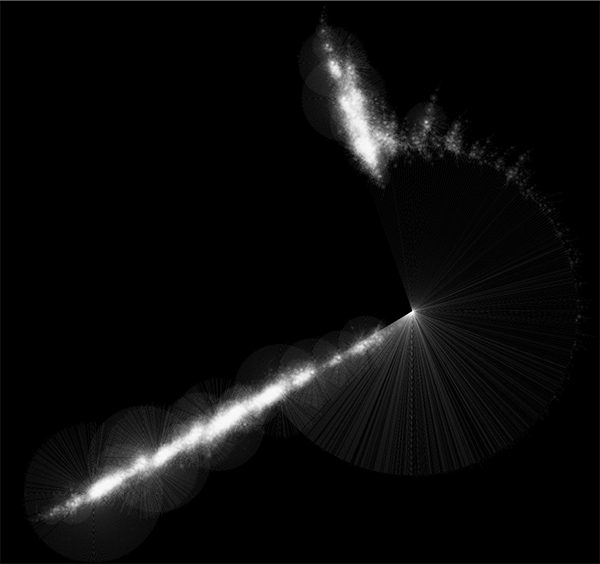
\includegraphics[width=\textwidth]{images/one_million_network.png}
		\end{figure}


\chapter{Cytoscape快速入门}
加载了网络之后,~Cytoscape~的界面如图~\ref{fig:2.1}~所示。

\begin{figure}[!h]
\centering
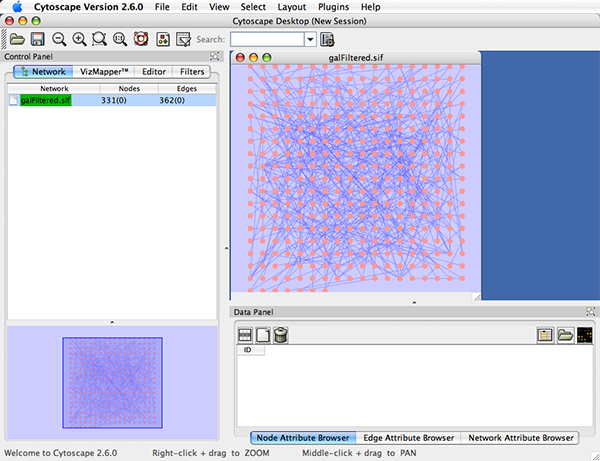
\includegraphics[width=\textwidth]{images/cytoscape_startup_network_26.png}
\caption{~Cytoscape~加载网络后的界面截图}
\label{fig:2.1}
\end{figure}

主界面由多个组件构成,包括:
\begin{itemize}
\item 顶部的菜单(稍后会对各个菜单做详细介绍)。
\item 工具栏,包含了各种常用功能。从菜单中也能使用这些功能。鼠标指针在这些图标上停留片刻就能看到有关的提示。
\item 网络管理面板(左上方的面板)。其中有可关闭的网络全局浏览面板(左下方)。
\item 网络查看主窗口,网络就显示在这个窗口中。
\item 属性浏览器面板(底部的面板),显示所选择的节点和边的属性。在这个面板中还可以对这些属性的值进行修改。
\end{itemize}

网络管理和属性浏览器面板是可以拖拽的标签面板,被称为~CytoPanels~。通过点击~CytoPanel~右上角的浮动窗口(Float Window)控件~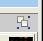
\includegraphics{images/float_icon.png}~可以将这些面板设为浮动状态。

如果选择了这个控件,例如属性浏览器面板上的这个控件,就会出现两个~Cytoscape~的窗口,一个是主窗口,另一个是名为CytoPanel 2的新窗口,如下图所示。当鼠标指针指向单元格时,会看到弹出信息。

{\centering
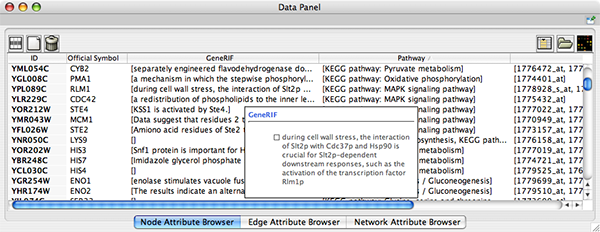
\includegraphics[width=\textwidth]{images/attribute_browser_26.png}
}

在图中可以看到,CytoPanel 2~现在有一个~Dock Window~控件。如果点选这个控件,这个窗口就会回到主窗口中。

Cytoscape~还提供了一个用于构建和编辑网络的编辑器,把面板中的节点和边拖拽到主网络视图窗口中就能创建和编辑网络。用Visual Style可以定义节点的形状以及边的箭头。只需要选择CytoPanel 1中的Editor标签就能编辑网络。下图展示了一个编辑器,Visual Style是BioMoleculeEditor。

{\centering
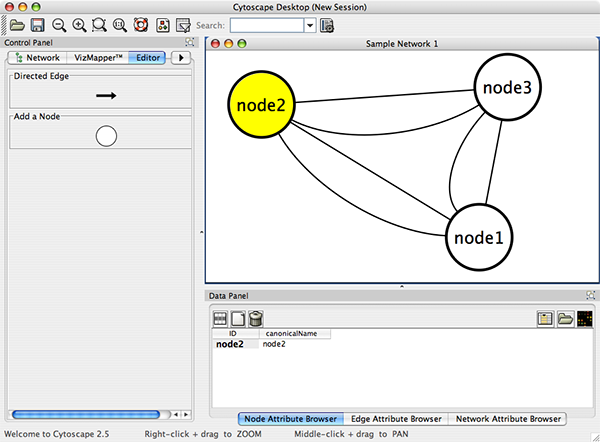
\includegraphics[width=\textwidth]{images/editor_25.png}}

\section{菜单}
	\subsection{File}
	File菜单中含有最基本的文件操作功能:File $\rightarrow$ Open~用于打开~Cytoscape~会话文件;File $\rightarrow$ New~用于新建空白网络,也可以从现用的网络创建新网络;File $\rightarrow$ Save~用于保存会话文件;File $\rightarrow$ Import~用于导入网络或属性数据;File $\rightarrow$ Export~用于导出数据和图片。File $\rightarrow$ Print用于打印,File $\rightarrow$ Quit~则是关闭所有的~Cytoscape~窗口,并推出程序。

	\begin{figure}[!h]
	\centerline{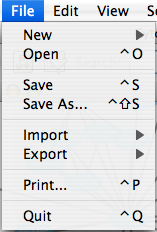
\includegraphics[scale=0.6]{images/menu_file_26.png} }
	\end{figure}

	\subsection{Edit}
	Edit菜单中提供了用于属性浏览器、网络编辑器和布局的撤销(Undo)和重做(Redo)功能。
	
	还有创建和销毁视图(网络的显示方法)和网络(网络的原始数据,并不可视化的)的菜单项,以及用于从当前网络中删除所选节点和边的菜单项。通过 Edit $\rightarrow$ Undo~可以恢复被删除的节点和边。配置和插件的设置可以通过Edit $\rightarrow$ Preferences $\rightarrow$ Properties来编辑。

	\begin{figure}[!h]
	\centerline{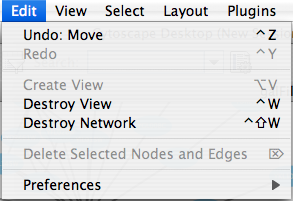
\includegraphics[scale=0.6]{images/menu_edit_26.png}}
	\end{figure}

	\subsection{View}
在~View~菜单中可以控制网络管理面板(CytoPanel 1)、属性浏览器(CytoPanel 2)、网络概览(在CytoPanel
1中)和VizMapper的显示和隐藏。

	\begin{figure}[!h]
	\centerline{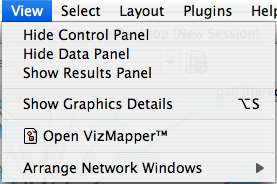
\includegraphics[scale=0.6]{images/menu_view_26.png}}
	\end{figure}

	\subsection{Select}
	在~Select~菜单中含有选择节点和边的各种选项。还有Select $\rightarrow$ Use Filter选项,用于根据节点或边的某些属性创建自动的过滤器。

	\begin{figure}[!h]
	\centerline{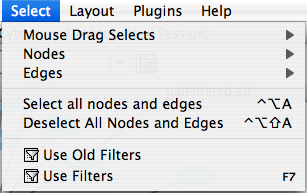
\includegraphics[scale=0.6]{images/menu_select_26.png}}
	\end{figure}

	\subsection{Layout}
	通过~Layout~菜单可以控制网络显示的形式。该菜单上半部分(Rotate,Scale,Align and
	 Distribute)是用于控制网络的显示。菜单的下半部分是用于自动布局网络的各种布局算法。

	\begin{figure}[!h]
	\centerline{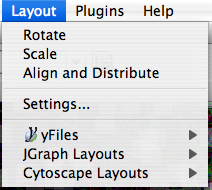
\includegraphics[scale=0.6]{images/menu_layout_25.png}}
	\end{figure}
	
		
	
	\subsection{Plugins}
	Plugins~菜单中提供了插件管理功能(安装、升级和删除),以及插件所添加的选项,比如
	~Agilent Literature Search~或~Merge Networks~。具体的内容取决于所加载的插件。
	\footnote{注意:在~\href{http://cytoscape.org/plugins2.php}
	{http://cytoscape.org/plugins2.php}~上有Cytoscape~插件的介绍。}
	
	\begin{figure}[!h]
	\centerline{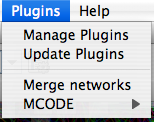
\includegraphics[scale=0.6]{images/menu_plugins_25.png}}
	\end{figure}
	
	\subsection{Help}
	在Help菜单中可以打开在线帮助,浏览本手册内容。“About...”则会显示正在运行的~Cytos
	cape~的版本信息。
	\begin{figure}[!h]
	\centerline{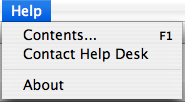
\includegraphics[scale=0.6]{images/menu_help_25.png}}
	\end{figure}

\section{网络管理}
	Cytoscape~2.3之后的版本都可以同时加载多个网络,有无视图都可以。网络中存放着用户
	加载所有节点和边,以及用户做指定的视图。同一个网络可以有多个视图。网络(以及相应
	的视图)可以有序地组织在一起。

    下图中展示了多个网络同时加载,并按层次结构组织的例子:

    \begin{figure}[!h]
    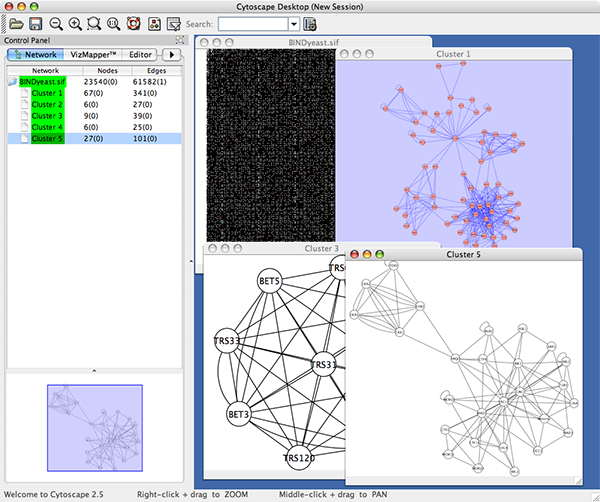
\includegraphics[width=\textwidth]{images/cytoscape_network_hierarchy_25.png}
    \end{figure}

    网络管理器(CytoPanel 1右上方的树状显示窗口)展示了当前所加载的网络。点击其中的
    网络就会在主窗口里面显示该网络的视图。在网络管理器中会显示各个网络的名称和尺寸(
    节点和边的数量)。如果网络是从文件中加载的,网络的名称就是文件名。
    
    对于那些规模较大的网络(数千个点和边),需要较长的时间才能显示出来。正因为如此, 
    Cytoscape中的网络可以不包含“视图”(View)。带有视图的网络以绿色高亮显示,而没有
    视图的网络则以红色高亮显示。在网络管理器中网络的名称上点击鼠标右键,就能创建或是
    销毁视图,通过Edit菜单也能实现同样的操作。用同样的方法可以销毁已加载的网络。在上
    图中,加载了七个网络,其中六个绿色的是有视图的,而红色的那个则是没有视图的 
    。\footnote{译者注:图中总共只有六个网络,都是绿色的,似乎原文有误。}

Cytoscape中的某些特定操作会创建出新的网络。如果新网络是从原有的网络中创建的,例如选择
原网络中的部分节点,将这些节点复制到新网络中(用File~$\to$~New~$\to$~Network option),
在这种情况下新网络就会显示为原网络的子网络。Cytoscape的这种显示方法使得用户能很快地
看出网络间的关系。上图中树顶部的那些网络就是这样生成的。

The available network views are also arranged as multiple overlapping windows in
the network view window. You can maximize, minimize, and destroy network views by
using the normal window controls for your operating system.

    \subsection{网络窗口排列}


\section{网络概览窗口}
	






\chapter{命令行参数}
Cytoscape~可以接受很多命令行参数,包括指定网络文件、属性文件和会话文件。下面的内容是用
Cytoscape~的“-h”或“--help”运行参数得到的:
\begin{verbatim}
usage: java -Xmx512M -jar cytoscape.jar [OPTIONS]
 -h,--help               Print this message.
 -v,--version            Print the version number.
 -s,--session <file>     Load a cytoscape session (.cys) file.
 -N,--network <file>     Load a network file (any format).
 -e,--edge-attrs <file>  Load an edge attributes file (edge attribute format).
 -n,--node-attrs <file>  Load a node attributes file (node attribute format).
 -m,--matrix <file>      Load a node attribute matrix file (table).
 -p,--plugin <file>      Load a plugin jar file, directory of jar files,
                         plugin class name, or plugin jar URL.
 -P,--props <file>       Load cytoscape properties file (Java properties
                         format) or individual property: -P name=value.
 -V,--vizmap <file>      Load vizmap properties file (Java properties format).
\end{verbatim}

在指定文件时,可以是本地文件的路径,也可以是URL。例如,可以这样指定本地的网络文件(假
设myNet.sif位于当前工作目录):cytoscape.sh -N myNet.sif。还可以用URL指定网络:
cytoscape.sh -N http://example.com/myNet.sif。
\begin{description}
\item[参数] 用途
\item[-h,--help] 显示上面已经展示过的帮助信息,然后退出程序。
\item[-v,--version] 显示~Cytoscape~的版本号,然后退出程序。

\item[-s,--session $<$file$>$] 这个选项用于加载指定的会话文件。
由于会话文件只能在特定的时间加载,所以这个选项在命令行中只能使用一次。要给这个选项指
定一个.cys~的~Cytoscape~会话文件。不过,cys~后缀并不是必须的。
\item[-N,--network $<$file$>$]
这个选项用来加载各种类型的网络文件,包括~SIG~、~GML~和~XGMML的各种格式的文件都可以通过- N
选项加载到~Cytoscape~中。在一个命令中可以同时加载多个网络。
\item[-e,--edge-attrs $<$file$>$] 这个选项用来指定边属性文件。
在一个命令中可以同指定多个边属性文件。
\item[-n,--node-attrs $<$file$>$] 这个选项用于指定节点属性文件。在一个命令中可以同指定多个边属性文件。
\item[-m,--matrix $<$file$>$]这个选项用于指定数据矩阵文件。
如果是用于生物网络分析,这个数据矩阵的内容就是基因表达数据。所有的数据矩阵文件都会以
节点属性的形式读入Cytoscape。在一个命令中可以同指定多个数据矩阵文件。
\item[-p,--plugin $<$file$>$]这个选项用于将指定的Cytoscape插件(.jar)文件加载到
Cytoscape中。老版本中的“资源插件选项(resource plugin option)”已经合并到了这个选项
中\footnote{这句话的翻译不确定,请有了解老版本Cytoscape的同学指正}。如果插件位于
Cytoscape的CLASSPATH路径中,还可以用类名称来制定插件。例如,假设能在~CLASSPATH~中找
到名为~MyPlugin~的类,那么就可以这样指定插件:cytoscape.sh -p MyPlugin.class。最后
一种指定插件的方面就是指定一个文本文件,在这个文本文件中列出所有需要加载的插件的~jar~文件名。 
\item[-P,--props
$<$file$>$]这个选项可以用来指定~Cytoscape~的各项属性。可以用过属性文件(格式是标准的
~Java~属性格式),也可以用等号设置单个属性的值。例如,指定缺省的物种:
cytoscape.sh -P defaultSpeciesName=Human。如果属性中有空格,加上引号就可以了,例如:
cytoscape.sh -P "defaultSpeciesName=Homo Sapiens"。
这个选项可以用来代替以前的-noCanonicalization,-species和-bioDataServer选项。现在的
命令可以写成这样的:cytoscape.sh -P defaultSpeciesName=Human -P noCanonicalization=true
-P bioDataServer=myServer.
\item[-V,--vizmap $<$file$>$] 这个选项用来指定可视化属性文件。
\end{description}

上面介绍的这些属性(包括插件)都可以在正在运行的Cytoscape的GUI中加载。




\end{CJK}
\end{document}

